%%% LaTeX Template
%%% This template can be used for both articles and reports.
%%%
%%% Copyright: http://www.howtotex.com/
%%% Date: February 2011

%%% Preamble
\documentclass[paper=a4, fontsize=11pt]{scrartcl}	% Article class of KOMA-script with 11pt font and a4 format

\usepackage[english]{babel}															% English language/hyphenation
\usepackage[protrusion=true,expansion=true]{microtype}				% Better typography
\usepackage{amsmath,amsfonts,amsthm}										% Math packages
\usepackage[pdftex]{graphicx}														% Enable pdflatex
%\usepackage{color,transparent}													% If you use color and/or transparency
\usepackage[hang, small,labelfont=bf,up,textfont=it,up]{caption}	% Custom captions under/above floats
\usepackage{epstopdf}																	% Converts .eps to .pdf
\usepackage{subfig}																		% Subfigures
\usepackage{booktabs}																	% Nicer tables
\usepackage{indentfirst}
\usepackage{hyperref}

%%% Advanced verbatim environment
\usepackage{verbatim}
\usepackage{fancyvrb}
\DefineShortVerb{\|}								% delimiter to display inline verbatim text


%%% Custom sectioning (sectsty package)
\usepackage{sectsty}								% Custom sectioning (see below)
\allsectionsfont{%									% Change font of al section commands
	\usefont{OT1}{bch}{b}{n}%					% bch-b-n: CharterBT-Bold font
%	\hspace{15pt}%									% Uncomment for indentation
	}

\sectionfont{%										% Change font of \section command
	\usefont{OT1}{bch}{b}{n}%					% bch-b-n: CharterBT-Bold font
	\sectionrule{0pt}{0pt}{-5pt}{0.8pt}%	% Horizontal rule below section
	}


%%% Custom headers/footers (fancyhdr package)
\usepackage{fancyhdr}
\pagestyle{fancyplain}
\fancyhead{}														% No page header
\fancyfoot[C]{\thepage}										% Pagenumbering at center of footer
\fancyfoot[R]{\small \texttt{exip v0.3}}	% You can remove/edit this line 
\renewcommand{\headrulewidth}{0pt}				% Remove header underlines
\renewcommand{\footrulewidth}{0pt}				% Remove footer underlines
\setlength{\headheight}{13.6pt}
\addtolength{\textheight}{0.7in}

%%% Equation and float numbering
\numberwithin{equation}{section}															% Equationnumbering: section.eq#
\numberwithin{figure}{section}																% Figurenumbering: section.fig#
\numberwithin{table}{section}																% Tablenumbering: section.tab#

\usepackage{url}
% ------------------------------------------------------------------------------
% Definitions (do not change this)
% ------------------------------------------------------------------------------
\newcommand{\HRule}[1]{\rule{\linewidth}{#1}} 	% Horizontal rule

\makeatletter							% Title
\def\printtitle{%						
    {\centering \@title\par}}
\makeatother									

\makeatletter							% Author
\def\printauthor{%					
    {\centering \large \@author}}				
\makeatother							

% ------------------------------------------------------------------------------
% Metadata (Change this)
% ------------------------------------------------------------------------------
\title{	\normalsize \textsc{EXIP - Embeddable EXI implementation in C} 	% Subtitle of the document
		 	\\[2.0cm]													% 2cm spacing
			\HRule{0.5pt} \\										% Upper rule
			\LARGE \textbf{\uppercase{EXIP User Guide}}	% Title
			\HRule{2pt} \\ [0.5cm]								% Lower rule + 0.5cm spacing
			\normalsize \today									% Todays date
		}

\author{
		\textbf{Rumen Kyusakov}\\	
		PhD student, Lule{\aa} University of Technology\\ [0.5cm]
		\HRule{0.5pt} \\ [0.5cm]
}

%%% Title	
%\title{ \vspace{-1in} 	\usefont{OT1}{bch}{b}{n}
%		\huge \strut This is the title of the template report \strut \\
%		\Large \bfseries \strut and a subtitle \strut
%}
%\author{ 									\usefont{OT1}{bch}{m}{n}
%        Firstname Lastname\\		\usefont{OT1}{bch}{m}{n}
%       University of Examples\\	\usefont{OT1}{bch}{m}{n}
%        Random Department\\
%        \texttt{email@example.com}
%}
%\date{}

%%% Begin document
\begin{document}
\thispagestyle{empty}				% Remove page numbering on this page

\printtitle									% Print the title data as defined above
  	\vfill
\begin{figure}[!h]
 \begin{center}
 
\includegraphics[width=0.70\textwidth, keepaspectratio=true]{images/logo.pdf} \\ [3.5cm]
\end{center}
\end{figure} 

\printauthor

\textit{Copyright (c) 2011, Rumen Kyusakov. This work is licensed under \href{http://creativecommons.org/licenses/by-sa/3.0/}{Creative Commons Attribution-ShareAlike 3.0 License}.}

\clearpage

\thispagestyle{empty}				% Remove page numbering on this page

\tableofcontents

\clearpage

\setcounter{page}{1}

\section{Introduction}

Add some introduction \cite{RumenKyusakov2011}



\section{Basic Concepts}
\label{sec:Basic-Concepts}

EXIP is a C library written in a portable manner that implements the EXI format for
XML representation. Probably a better way of describing what is EXIP is to say what it is \emph{not}.
EXIP is not a tool for converting text XML documents to EXI and vice versa. Why is that then?
To start with, the XML to EXI conversion requires a XML parser that process the XML input.
The XML parser itself is at least as big chunk of code as it is the EXI parser and having them
both at the same time might not be
possible or desired on a resource constrained embedded system. Second, parsing
the text XML and then converting it to EXI effectively removes all the processing benefits of EXI.
Having said that, it does not mean that it is not possible to use EXIP in such scenario. For example,
it is planned as a future work to include a module in EXIP that performs exactly that: generating
corresponding EXI streams from a text XML input and vice versa. It is therefore an optional
behavior and not an only possible way of using the library. It is not even difficult to implement
such a module and the reader could do that as a practical exercise after going through this guide.

As a result of this design choice, EXIP cannot use (at least for now) the XML Schema format directly
to perform schema-enabled processing. This might sound as a big flaw in the implementation but is
just the opposite. XML Schema documents are plain XML documents and as such they have analogous EXI
representation. Working with the EXI representation of the XML Schema definitions brings all the
performance benefits of the EXI itself - faster processing and more compact representation.
Now, using static systems where the schema information is only processed at design time would
not make much difference. However, once you are faced with more dynamic systems that are
capable of handling schema information at run-time, the use of EXI representation is more
beneficial especially in networked embedded environments.

Yet another \emph{not} - EXIP is not compliant with DOM, SAX or StAX Application Programming Interfaces (APIs)
for XML processing. The single reason for that is the efficiency trade-off. All these APIs are
using string representation of the primitive data types defined by the XML Schema specification
such as float, integer, date etc. This means that when schema definitions are available these
types must be converted from native types to string and then back from string to native representation
in order to fit in the API. Once again this does not mean that you cannot use EXIP with applications
that require DOM, SAX or StAX interface. The EXIP API is low level and typed and requires a
wrapper module in order to provide the aforementioned interfaces, which again is scheduled for future work.

\begin{figure}[h!]
 \begin{center}
 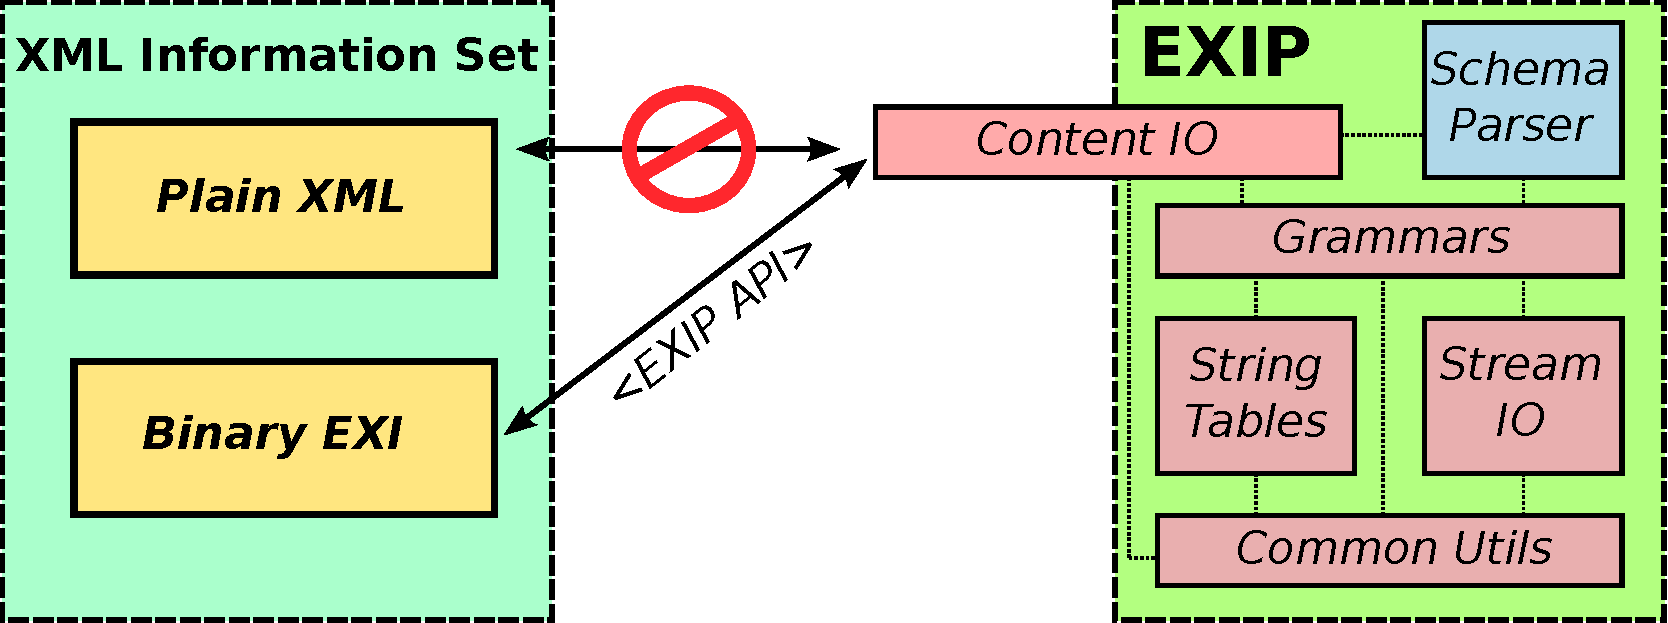
\includegraphics[width=0.90\textwidth, keepaspectratio=true]{images/EXIP-overview.pdf}
\end{center}
\caption{EXIP components}
\label{fig:EXIP-components} 
\end{figure} 

Figure \ref{fig:EXIP-components} depicts these design decisions and shows the different components of
the library. Key concept when creating the structure of the project was modularity - the functionality
is grouped and encapsulated in different components. This allows for disabling features that are not
needed directly at compile time. As an example, the Schema Parser component that is responsible for
generation the grammar structures based on XML Schema definitions is only needed if the system is
expected to dynamically handle XML schemes and hence in all other cases can be removed from the build at compile time. 

For further information and details on the EXIP API and the rational
behind it see the paper that first presents EXIP \cite{RumenKyusakov2011} (please refer to this work when 
citing information from this guide or other EXIP documentation).

\subsection{Project structure}
\label{sec:project-structure}

The EXIP library is an Eclipse C project (and MS Visual Studio 2010 solution)
structured in the following subdirectories:
\begin{itemize}
 \item \texttt{bin/} - this is the build output directory. It is automatically created/removed when
doing builds of the project. The library binaries are located directly into the \texttt{bin/} folder
while the examples and other utils are compiled in separate subfolders

 \item \texttt{build/} - this folder contains the build scripts of the project. The current release
provides a MS VS 2010 build under \texttt{build/vs2010/} and \emph{GCC} toolchain builds under \texttt{build/gcc/}.
The \texttt{build/gcc/} folder further contains platform-dependent parameters and
headers located in subfolders - \texttt{build/gcc/mulle} for the Mulle sensor platform,
\texttt{build/gcc/oe-armv5te} for OpenEmbedded Linux on ARMv5te and the default
\texttt{build/gcc/pc} for descktop PCs. The build is started from \texttt{build/gcc/} with the following
\texttt{make} build targets available:
\begin{description}
 \item[all] compiles the EXIP library. The default target platform is PC. To change the target
platform to Mulle for example, add \texttt{target=mulle} as an argument of \texttt{make}
 \item[check] invokes the Check unit tests
 \item[clean] removes the \texttt{bin/} folder
 \item[doc] generates the project Doxygen documentation. The output directory is set to \texttt{doc/dev/doxygen/}
 \item[examples] compiles and builds the example executables
 \item[utils] compiles and builds the utils executables
 \item[lib] generates a static library libexip.a in \texttt{bin/lib}
 \item[dynlib] generates a dynamic library libexip.so in \texttt{bin/lib}
 \end{description}

 \item \texttt{doc/} - the project documentation: \texttt{doc/user/} contains the source of this user guide;
    \texttt{doc/dev/} is the development documentation; 
  \texttt{doc/www/} contains the information available on the project web page

 \item \texttt{examples/} - the root of the example applications shipped with EXIP

 \item \texttt{include/} - this folder contains the public header files of the EXIP library.
			  Together with the \texttt{exipConfig.h} defined per target platform, these files
			  define the public interface of the library.

 \item \texttt{src/} - here are all internal definitions and \texttt{.c} files divided into
	      subfolders according to the modules in which they belong

 \item \texttt{tests/} - Check unit tests, integration and validation tests

 \item \texttt{utils/} - supporting utilities and development tools

\end{itemize}


\subsection{Strings in EXIP}
\label{sec:strings}

All character strings in EXIP are length prefixed. This means that all the strings that are passed to
the EXI encoder and all the strings that are parsed from the decoder are in this format. The motivation
for that is the number of string comparisons that the EXI processor must perform when going through an
EXI stream. In many cases, when the strings differ in length, this operation is very efficient
when the length is saved together with the characters data. EXIP provides an API for working with
this type of strings defined in \texttt{stringManipulate.h}. The implementation of the functions
declared in this header file defines what type of characters are supported in the string.
For example, \texttt{ASCII\_stringManipulate.c} implements the strings as ASCII character arrays.

One way of increasing the compactness defined in the EXI specification is through the use of string tables.
The string tables are partitioned dictionary that stores and indexes the strings that occur in particular
EXI document. In such way, when a string has been used once in the document it is added to the string tables.
Every other occurrence of the same string in the document is represented by its index in the string tables.

\begin{figure}[h!]
 \begin{center}
 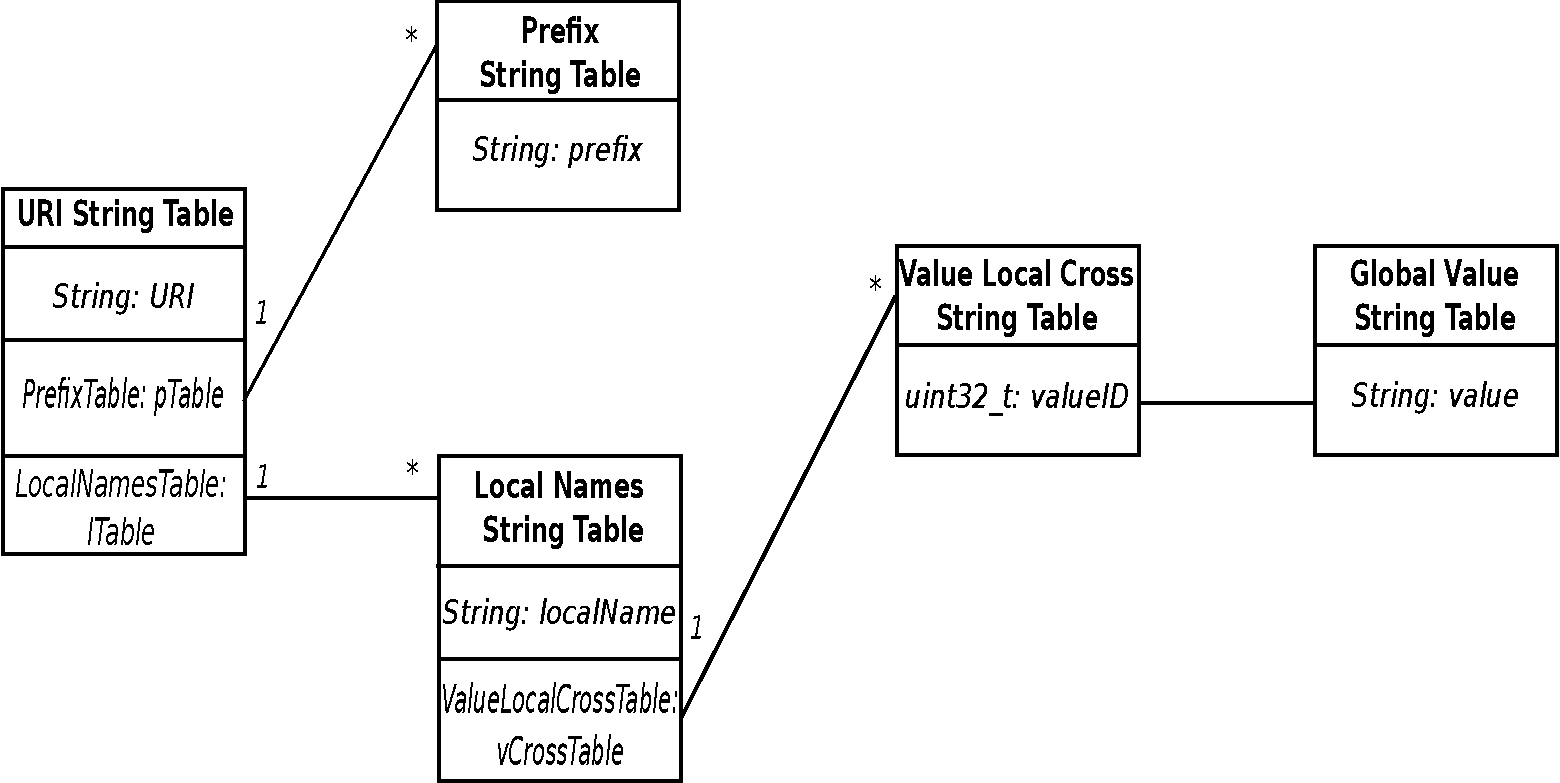
\includegraphics[width=0.90\textwidth, keepaspectratio=true]{images/StringTablesDiag.pdf}
\end{center}
\caption{String tables in EXIP}
\label{fig:EXIP-string-tables} 
\end{figure} 

Figure \ref{fig:EXIP-string-tables} shows how the string tables are implemented in EXIP. As a user of
the library you do not need to understand the actual implementation details. The only thing that you need
to be aware of is that the strings that are passed to your application by the EXIP parser should not be
modified as they are integral part of the string tables. You can clone the strings and use that copy
for string manipulations.

\subsection{Error handling and memory management}
\label{sec:errors-memory}
When an invalid input is given to the EXIP parser or some other error conditions occur, the
EXIP library functions return a numeric error codes that are defined in \texttt{errorHandle.h}.
More fine-grained error messages can be acquired by turning on the debugging routines.
You have control over the level of verbosity (INFO, WARNING or ERROR) and the source of
debugging information. All these parameters can be configured in the \texttt{exipConfig.h} header
that is defined per target platform in \texttt{build/gcc/<target\_platform>} or
\texttt{build/vs2010} for Windows.
When turned on the debugging information is by default printed on the standard output.

EXIP has an internal memory management infrastructure and you are not required to
know its details unless you are using the EXIP string type in your own applications. That is because
the string manipulation functions use \texttt{AllocList} to manage their allocations.
You can either define your own string manipulation functions or acquaint yourself with 
the memory management routines defined in \texttt{memManagement.h}.


\section{Maturity Statement}
\label{sec:Maturity-Statement}

The latest release of the EXIP library is pre-alpha version 0.3. As such, 
many features are missing and others are not stable enough for real-world
usage. Here is the status of the EXIP functionality:

\begin{itemize}
 \item Currently only ASCII strings are supported. It should be relatively easy to extend
that with Unicode strings by implementing a dozen of functions in the header
file \texttt{stringManipulate.h}
 \item EXIP is working quite stable when using the default options in the EXI header in schema-less mode
 \item Schema-enabled mode is unstable and has limited features supported. The reason is in the
status of the grammar generation utility that converts XML Schema definitions to EXIP grammars.
For example, the import of external schema definitions through \texttt{xsd:import} is currently not supported.
 \item The following EXI header options are supported: EXI Cookie, Options Presence Bit, Strict, Fragment,
Preserve.prefixes, SchemaId, ValueMaxLength and ValuePartitionCapacity.
\end{itemize}

\section{Serialization}

Describe the serialization step by step


\section{Parsing}
\label{sec:Parsing}

The parsing interface of EXIP is similar to SAX and StAX. The main difference is
that most of the XML schema build-in types are passed in a native binary form
rather than as a string representation.
The EXIP parser processes the EXI stream in one direction and produces events
on occurrence of information items such as elements, attributes or content values.
The applications using EXIP must register callback functions for the events that they are interested in.
In this way the data from the EXI stream is delivered to the application as a
parameters to these callback functions.
The header \texttt{contentHandler.h} provides declarations of the callback functions
while the API for controlling the progress through the EXI stream is in \texttt{EXIParser.h}.

\subsection{Schema-less decoding}

When in schema-less mode all value items are encoded with strings and hence
delivered to the application through the \texttt{stringData()} callback handler.
Similarly to the serialization, the parsing consists of 7 simple steps:
\begin{enumerate}
 \item Declare a parser container that holds the serialized data and EXIP state:
\begin{lstlisting}
Parser parser;
\end{lstlisting}

 \item Define a binary input buffer for reading the EXI stream.
The buffer can optionally include an external input stream for fetching the
serialized EXI data. If an input stream is not defined the whole EXI
document must be stored in memory before starting the
parsing process. The following code declares and initializes an input memory buffer:
\begin{lstlisting}
BinaryBuffer buffer;
char buf[INPUT_BUFFER_SIZE];

buffer.buf = buf;
buffer.bufLen = INPUT_BUFFER_SIZE;
buffer.bufContent = 0;
\end{lstlisting}
Beside these definitions, when a file is used to fetch the
EXI data the following steps are also required: 
\begin{lstlisting}
/* IN CASE OF FILE INPUT STREAM */
/* Define a function implementing the actual reading from a file */
size_t readFromFileInputStream(void* buf, size_t readSize, void* stream)
{
	FILE *infile = (FILE*) stream;
	return fread(buf, 1, readSize, infile);
}

FILE *infile; /* Using a file for fetching the EXI data */
infile = fopen(sourceEXIFile, "rb" ); /* open the file before use */
buffer.ioStrm.readWriteToStream = readFromFileInputStream;
buffer.ioStrm.stream = infile; /* Sets the input stream to the file */
\end{lstlisting}
If no file or other input streams are being used (e.i. the whole EXI message is
stored in \texttt{buffer.buf}), the input function and the stream
of the \texttt{BinaryBuffer} must be initialized with NULL values:
\begin{lstlisting}
/* IN CASE OF IN-MEMORY ONLY INPUT*/
buffer.ioStrm.readWriteToStream = NULL;
buffer.ioStrm.stream = NULL;
\end{lstlisting}

The size of the \texttt{INPUT\_BUFFER\_SIZE} macro depends on the
use case. When in in-memory input mode or sufficient RAM on the
platform the buffer size should be kept high. Note that even if
an input stream is used such as a file, a non-zero length buffer
for temporary storing parts of the EXI data is still needed.

 \item Define application data and initialize the parser object:
\begin{lstlisting}
/** The application data that is passed to the callback handlers*/
struct applicationData
{
  unsigned int elementCount;
  unsigned int nestingLevel;
} appData;

/**
 * @param[in, out] parser EXIP parser container
 * @param[in] buffer binary buffer for fetching EXI encoded data
 * @param[in] NULL a compiled schema information to be used for schema
		      enabled processing; NULL if no schema is available
 * @param[in, out] appData application data to be passed to the callback handlers
 */  
initParser(&parser, buffer, NULL, &appData);    
\end{lstlisting}

 \item Initialize the application data and register the callback handlers with the parser object:
\begin{lstlisting}
appData.elementCount = 0; /* Example: the number of elements passed */
appData.nestingLevel = 0; /* Example: the nesting level */

parser.handler.fatalError = sample_fatalError;
parser.handler.error = sample_fatalError;
parser.handler.startDocument = sample_startDocument;
parser.handler.endDocument = sample_endDocument;
parser.handler.startElement = sample_startElement;
parser.handler.attribute = sample_attribute;
parser.handler.stringData = sample_stringData;
parser.handler.endElement = sample_endElement;

/** According to the above definitions:
  *  When the parser start parsing the body, the sample_startDocument()
  *  callback will be invoked; when a start of an element is parsed the
  *  sample_startElement() will be invoked and so on. All of the events
  *  for which there is no handler registered will be discarded. 
  */
\end{lstlisting}

 \item Parse the header of the stream:
\begin{lstlisting}
parseHeader(&parser);
/* The header fields are stored in parser.strm.header*/
\end{lstlisting}

 \item Parse the body of the EXI stream, one content item at a time:
\begin{lstlisting}
errorCode error_code = ERR_OK;
while(error_code == ERR_OK)
{
  error_code = parseNext(&parser);
}

/**
 * On successful parsing step, the parseNext() returns ERR_OK if there
 * are more content items left for parsing and PARSING_COMPLETE in case
 * the parsing is complete. If error conditions occur during the
 * process it returns an error code.
 */
\end{lstlisting}

 \item Destroy the parser object and free the memory allocated by it. If any other
streams are left open close them as well:
\begin{lstlisting}
destroyParser(&parser);
fclose(infile);
\end{lstlisting}

\end{enumerate}
\subsection{Schema-enabled decoding}
When in schema-enabled mode the basic parsing steps are essentially the same.
The difference is in the \texttt{EXIPSchema*} parameter passed to the \texttt{initParser()}.
You need to pass a valid \texttt{EXIPSchema} object and not NULL as in the schema-less
case. This object contains all the definitions and constrains from the XML schema and
its creation is a topic of section \ref{sec:Schema-Infromation} \textbf{Schema Information}.
During parsing, the value types as defined by the schema definitions
are delivered through the corresponding callback handlers and not only \texttt{stringData()}.
For example, \texttt{xsd:integer} is delivered through \texttt{intData()} and
\texttt{xsd:boolean} through \texttt{booleanData()}. Apart from that all other decoding steps
are the same as in schema-less mode.

\section{Schema Information}
\label{sec:Schema-Infromation}

This section examines the different ways of construction \texttt{EXIPSchema} object
containing the XML schema definitions and constrains. The header \texttt{grammarGenerator.h}
defines a single function that takes a XML schema document(s) and convert them to 
\texttt{EXIPSchema} object. This function can be used to dynamically (at run-time)
parse a schema and generate the needed EXIP constructs for schema-enabled
EXI parsing and serialization. As mentioned earlier, the EXIP library currently supports
only XML schema definitions represented in EXI format. Moreover, the fidelity option \texttt{Preserve.prefixes} must be
set in order to decode the QNames in the value items correctly (see the EXI specification for
more information on that).

When the XML schemes are static (only used at
compile time) the \texttt{grammarGen} module is not needed and can be excluded from the build.
In this case the \texttt{EXIPSchema} object can be build from automatically generated source code
by the \texttt{exipg} utility implemented in \texttt{utils/schemaHandling/createGrammars.c}.

\subsection{Using exipg utility}
The \texttt{exipg} utility is a command line tool for generating EXI grammar definitions
for schema-enabled EXI processing based on XML schemes.
It is using grammar generation
function in \texttt{grammarGenerator.h} and as such also requires EXI encoded XML schemes.
There are three modes defining the output of the tool:
\begin{description}
 \item[exip] In this mode the XML schema is serialized into an EXIP specific format. The output is
	    an EXI document that later can be loaded into the EXIP library for schema-enabled processing.
	    This option is not implemented currently.
 \item[text] In this mode the grammar definitions are printed in human readable form. This mode is
	    useful for debugging purposes.
 \item[src] In this mode the grammar definitions are generated in \texttt{C} source code. The code
	    can use either static definitions (everything is in the programming memory) or
	    dynamic definitions (dynamic memory allocations).
 \end{description}
As an example, the command line arguments used to generate the EXI Options document grammars are:
\begin{lstlisting}
exipg -src=static -pfx=ops_ -mask=1000000 EXIOptions-xsd.exi staticEXIOptions.c
\end{lstlisting}

\subsection{Converting XML Schema files to EXI}
Currently, there are not any XML Schema editing tools that are capable of saving the document in EXI format.
For that reason it is required that you convert the text XML Schema to EXI encoding before using it
with EXIP. You can use any of the open source Java implementations of EXI for that purpose. Particularly
convenient for use is the \href{http://sourceforge.net/projects/exiprocessor/files/}{ExiProcessor} command line utility.
The correct arguments to be passed to the utility for converting the EXIOptions.xsd are:
\begin{lstlisting}
java -jar ExiProcessor.jar -header_options -preserve_prefixes
  -xml_in EXIOptions.xsd -exi_out EXIOptions-xsd.exi
\end{lstlisting}

\bibliographystyle{IEEEtran}
\bibliography{references}
\end{document}